\documentclass[12pt,]{article}
\usepackage{lmodern}
\usepackage{amssymb,amsmath}
\usepackage{ifxetex,ifluatex}
\usepackage{fixltx2e} % provides \textsubscript
\ifnum 0\ifxetex 1\fi\ifluatex 1\fi=0 % if pdftex
  \usepackage[T1]{fontenc}
  \usepackage[utf8]{inputenc}
\else % if luatex or xelatex
  \ifxetex
    \usepackage{mathspec}
    \usepackage{xltxtra,xunicode}
  \else
    \usepackage{fontspec}
  \fi
  \defaultfontfeatures{Mapping=tex-text,Scale=MatchLowercase}
  \newcommand{\euro}{€}
\fi
% use upquote if available, for straight quotes in verbatim environments
\IfFileExists{upquote.sty}{\usepackage{upquote}}{}
% use microtype if available
\IfFileExists{microtype.sty}{%
\usepackage{microtype}
\UseMicrotypeSet[protrusion]{basicmath} % disable protrusion for tt fonts
}{}
\usepackage[margin=1in]{geometry}
\usepackage{graphicx}
\makeatletter
\def\maxwidth{\ifdim\Gin@nat@width>\linewidth\linewidth\else\Gin@nat@width\fi}
\def\maxheight{\ifdim\Gin@nat@height>\textheight\textheight\else\Gin@nat@height\fi}
\makeatother
% Scale images if necessary, so that they will not overflow the page
% margins by default, and it is still possible to overwrite the defaults
% using explicit options in \includegraphics[width, height, ...]{}
\setkeys{Gin}{width=\maxwidth,height=\maxheight,keepaspectratio}
\ifxetex
  \usepackage[setpagesize=false, % page size defined by xetex
              unicode=false, % unicode breaks when used with xetex
              xetex]{hyperref}
\else
  \usepackage[unicode=true]{hyperref}
\fi
\hypersetup{breaklinks=true,
            bookmarks=true,
            pdfauthor={},
            pdftitle={Is the Tea Party Libertarian, Authoritarian, or Something Else?},
            colorlinks=true,
            citecolor=black,
            urlcolor=red,
            linkcolor=black,
            pdfborder={0 0 0}}
\urlstyle{same}  % don't use monospace font for urls
\setlength{\parindent}{0pt}
\setlength{\parskip}{6pt plus 2pt minus 1pt}
\setlength{\emergencystretch}{3em}  % prevent overfull lines
\setcounter{secnumdepth}{0}

%%% Change title format to be more compact
\usepackage{titling}
\setlength{\droptitle}{-2em}
  \title{Supplementary Information for ``Is the Tea Party Libertarian, Authoritarian, or Something Else?''
\vspace{1.25em}}
  \pretitle{\vspace{\droptitle}\centering\huge}
  \posttitle{\par}
  \author{}
  \preauthor{}\postauthor{}
  \date{}
  \predate{}\postdate{}


\usepackage{setspace}


\begin{document}

\maketitle

\paragraph{Contents}\label{contents}

\begin{enumerate}
\def\labelenumi{\arabic{enumi}.}
\itemsep1pt\parskip0pt\parsep0pt
\item
  Scree plot for factor model
\item
  Numerical factor loadings
\item
  Including Party ID as a covariate
\item
  Estimated effects of misarchism on Party ID and Conservatism
\item
  Probabilities of covariate inclusion from Bayesian Model Averaging
\item
  Expected value of coefficients from Bayesian Model Averaging
\item
  Pooled regression results after multiple imputation
\item
  Multiple imputation diagnostics
\end{enumerate}

\begin{figure}[htbp]
\centering
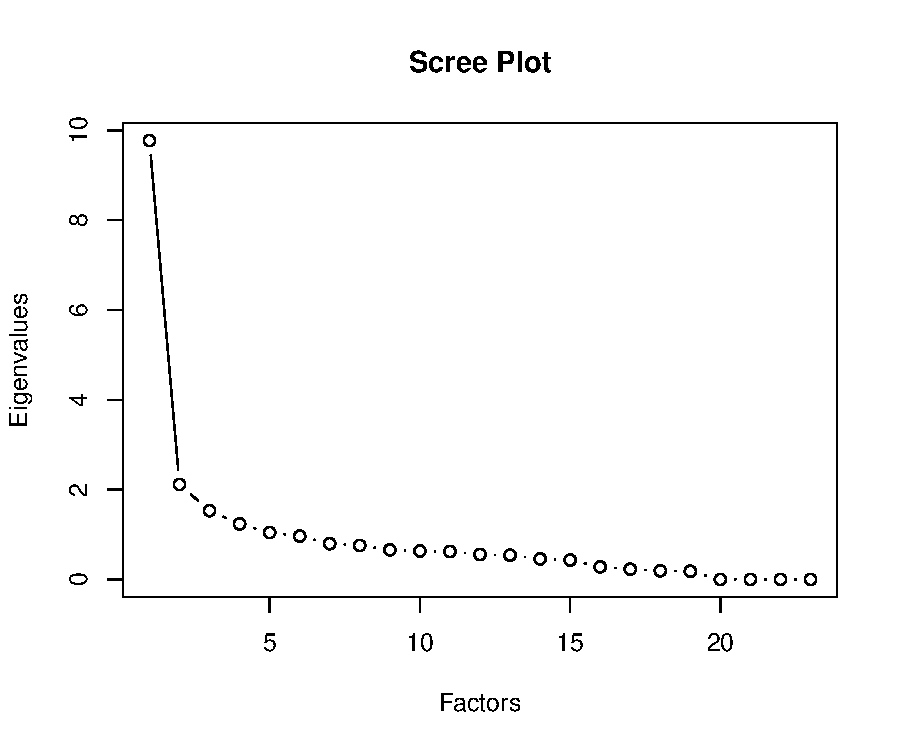
\includegraphics{figures/scree-1.pdf}
\caption{Biplot shows two main dimensions}
\end{figure}

\clearpage

\begin{table}[ht]
\centering
\begin{tabular}{rrr}
  \hline
 & Moral Statism & Governmentalism \\ 
  \hline
Conservatism & 0.56 & -0.26 \\ 
  Family & 0.64 & 0.08 \\ 
  GunControl & -0.06 & 0.39 \\ 
  Intolerant & 0.42 & -0.12 \\ 
  Morals & 0.35 & -0.21 \\ 
  Wiretapping & 0.37 & 0.24 \\ 
  DefenseSpending & 0.54 & 0.08 \\ 
  Services & -0.00 & 0.77 \\ 
  ImmigrationChecks & 0.39 & -0.21 \\ 
  JobGuarantee & -0.06 & 0.60 \\ 
   \hline
\end{tabular}
\caption{Factor Loadings} 
\label{Factor Loadings}
\end{table}

\clearpage

\begin{table}[!htbp] \centering 
  \caption{Alternative Dependent Variables for Model 2} 
  \label{} 
\footnotesize 
\begin{tabular}{@{\extracolsep{5pt}}lcc} 
\\[-1.8ex]\hline 
\hline \\[-1.8ex] 
 & \multicolumn{2}{c}{\textit{Dependent variable:}} \\ 
\cline{2-3} 
\\[-1.8ex] & PartyID (Republican) & Conservatism \\ 
\\[-1.8ex] & (1) & (2)\\ 
\hline \\[-1.8ex] 
 Gender (Male) & $-$0.005 & 0.005 \\ 
  & (0.013) & (0.011) \\ 
  Income & 0.033$^{**}$ & $-$0.002 \\ 
  & (0.015) & (0.013) \\ 
  Age & $-$0.068$^{***}$ & $-$0.029$^{**}$ \\ 
  & (0.014) & (0.012) \\ 
  Race (White) & 0.066$^{***}$ & $-$0.053$^{***}$ \\ 
  & (0.016) & (0.013) \\ 
  Education & 0.047$^{***}$ & 0.005 \\ 
  & (0.015) & (0.013) \\ 
  Obama & $-$0.549$^{***}$ & 0.068$^{***}$ \\ 
  & (0.020) & (0.020) \\ 
  Authoritarianism & $-$0.037$^{**}$ & $-$0.031$^{**}$ \\ 
  & (0.015) & (0.013) \\ 
  BornAgain & 0.014 & $-$0.007 \\ 
  & (0.014) & (0.012) \\ 
  Religion & 0.002 & 0.003 \\ 
  & (0.015) & (0.013) \\ 
  PartyID (Republican) &  & 0.172$^{***}$ \\ 
  &  & (0.017) \\ 
  FoxNews & 0.043$^{***}$ & 0.014 \\ 
  & (0.015) & (0.013) \\ 
  MoralStatism & 0.198$^{***}$ & 0.748$^{***}$ \\ 
  & (0.026) & (0.022) \\ 
  Government & $-$0.131$^{***}$ & $-$0.089$^{***}$ \\ 
  & (0.024) & (0.021) \\ 
  MoralStatism*Government & 0.022 & 0.060$^{***}$ \\ 
  & (0.027) & (0.023) \\ 
  Constant & $-$0.045$^{**}$ & 0.036$^{**}$ \\ 
  & (0.020) & (0.017) \\ 
 \hline \\[-1.8ex] 
Observations & 2,406 & 2,406 \\ 
R$^{2}$ & 0.661 & 0.712 \\ 
Adjusted R$^{2}$ & 0.659 & 0.710 \\ 
Residual Std. Error & 0.311 (df = 2392) & 0.266 (df = 2391) \\ 
F Statistic & 359.000$^{***}$ (df = 13; 2392) & 422.000$^{***}$ (df = 14; 2391) \\ 
\hline 
\hline \\[-1.8ex] 
\textit{Note:}  & \multicolumn{2}{r}{$^{*}$p$<$0.1; $^{**}$p$<$0.05; $^{***}$p$<$0.01} \\ 
\end{tabular} 
\end{table}

\begin{table}[!htbp] \centering 
  \caption{Including Party ID as a Covariate} 
  \label{} 
\footnotesize 
\begin{tabular}{@{\extracolsep{5pt}}lc} 
\\[-1.8ex]\hline 
\hline \\[-1.8ex] 
 & \multicolumn{1}{c}{\textit{Dependent variable:}} \\ 
\cline{2-2} 
\\[-1.8ex] & Tea Party Support \\ 
\hline \\[-1.8ex] 
 Gender (Male) & 0.132 \\ 
  & (0.129) \\ 
  Income & $-$0.322$^{**}$ \\ 
  & (0.148) \\ 
  Conservatism & 0.785$^{***}$ \\ 
  & (0.255) \\ 
  Age & $-$0.354$^{**}$ \\ 
  & (0.145) \\ 
  Race (White) & $-$0.419$^{**}$ \\ 
  & (0.168) \\ 
  Education & 0.057 \\ 
  & (0.159) \\ 
  Obama & $-$1.350$^{***}$ \\ 
  & (0.224) \\ 
  Authoritarianism & 0.052 \\ 
  & (0.148) \\ 
  BornAgain & 0.288$^{**}$ \\ 
  & (0.135) \\ 
  Religion & $-$0.027 \\ 
  & (0.156) \\ 
  PartyID (Republican) & 0.313 \\ 
  & (0.202) \\ 
  FoxNews & 0.682$^{***}$ \\ 
  & (0.134) \\ 
  MoralStatism & 0.093 \\ 
  & (0.337) \\ 
  Government & $-$0.670$^{**}$ \\ 
  & (0.265) \\ 
  MoralStatism*Government & $-$1.510$^{***}$ \\ 
  & (0.321) \\ 
  Constant & $-$2.570$^{***}$ \\ 
  & (0.208) \\ 
 \hline \\[-1.8ex] 
Observations & 2,406 \\ 
Log Likelihood & $-$828.000 \\ 
Akaike Inf. Crit. & 1,688.000 \\ 
\hline 
\hline \\[-1.8ex] 
\textit{Note:}  & \multicolumn{1}{r}{$^{*}$p$<$0.1; $^{**}$p$<$0.05; $^{***}$p$<$0.01} \\ 
\end{tabular} 
\end{table}

\clearpage

\begin{figure}[htbp]
\centering
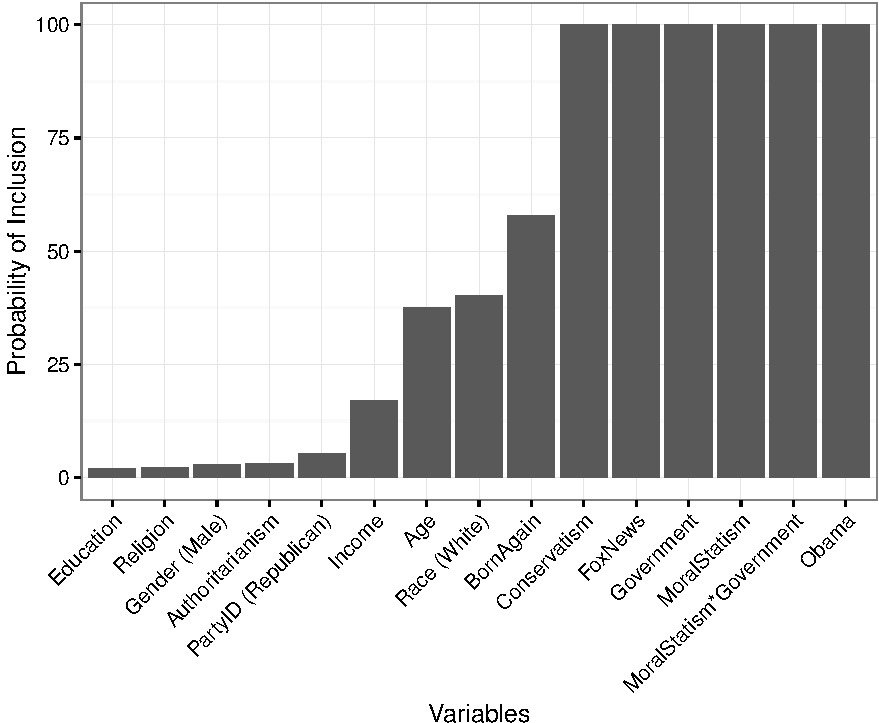
\includegraphics{figures/bma2-1.pdf}
\caption{Inclusion Probabilites from Bayesian Model Averaging}
\end{figure}

\clearpage

\begin{figure}[htbp]
\centering
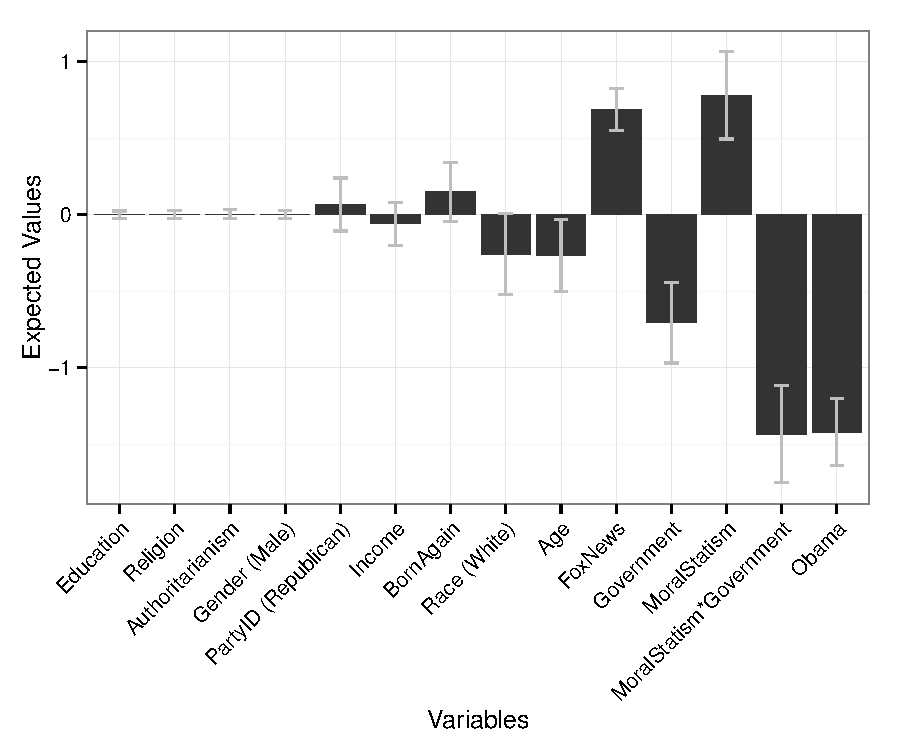
\includegraphics{figures/bma3-1.pdf}
\caption{Expected Values from Bayesian Model Averaging}
\end{figure}

\clearpage

\begin{table}[ht]
\centering
\begin{tabular}{rrrrr}
  \hline
 & Value & Std. Error & t-stat & p-value \\ 
  \hline
(Intercept) & -2.08 & 0.12 & -18.04 & 0.00 \\ 
  Gender (Female) & -0.10 & 0.09 & -1.12 & 0.26 \\ 
  Income & -0.33 & 0.10 & -3.33 & 0.00 \\ 
  Age & -0.30 & 0.09 & -3.38 & 0.00 \\ 
  Race (White) & -0.30 & 0.11 & -2.68 & 0.01 \\ 
  Education & -0.04 & 0.10 & -0.43 & 0.66 \\ 
  Obama & -0.99 & 0.14 & -7.04 & 0.00 \\ 
  Authoritarianism & 0.06 & 0.11 & 0.60 & 0.55 \\ 
  BornAgain & -0.21 & 0.12 & -1.77 & 0.08 \\ 
  Religion & 0.02 & 0.09 & 0.19 & 0.85 \\ 
  PartyID (Republican) & 0.23 & 0.13 & 1.75 & 0.08 \\ 
  FoxNews & 0.66 & 0.10 & 6.90 & 0.00 \\ 
  MoralStatism & 0.98 & 0.18 & 5.35 & 0.00 \\ 
  Government & -0.67 & 0.17 & -4.03 & 0.00 \\ 
  MoralStatism*Government & -1.34 & 0.20 & -6.76 & 0.00 \\ 
   \hline
\end{tabular}
\caption{Pooled Logistic Regression Results From 10 Multiple Imputations} 
\end{table}

\clearpage

\begin{figure}[htbp]
\centering
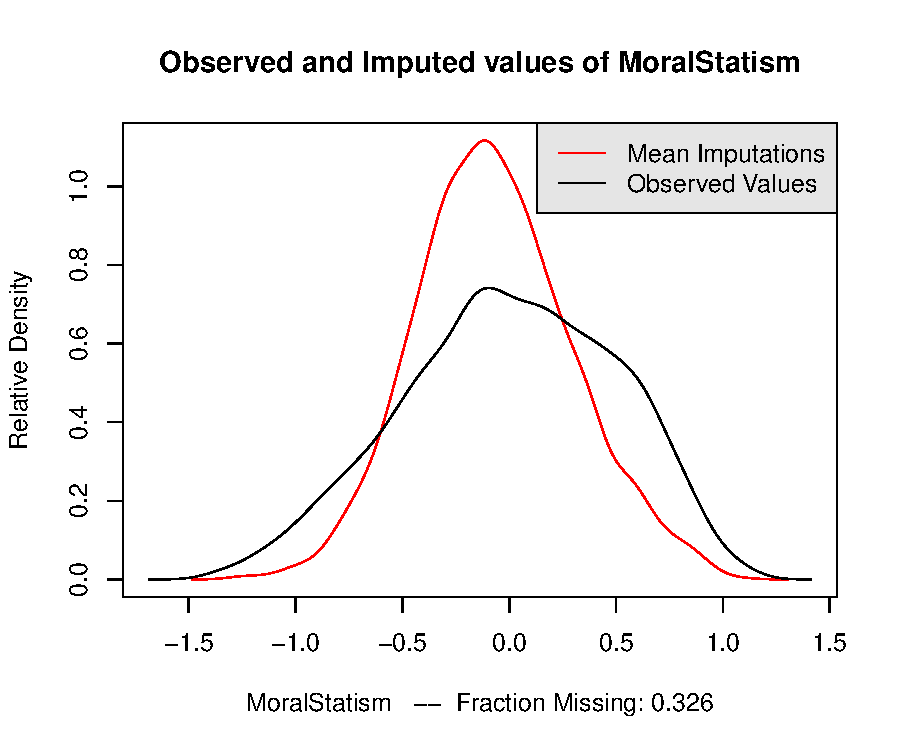
\includegraphics{figures/missing2-1.pdf}
\caption{Distributions before and after multiple imputation}
\end{figure}

\begin{figure}[htbp]
\centering
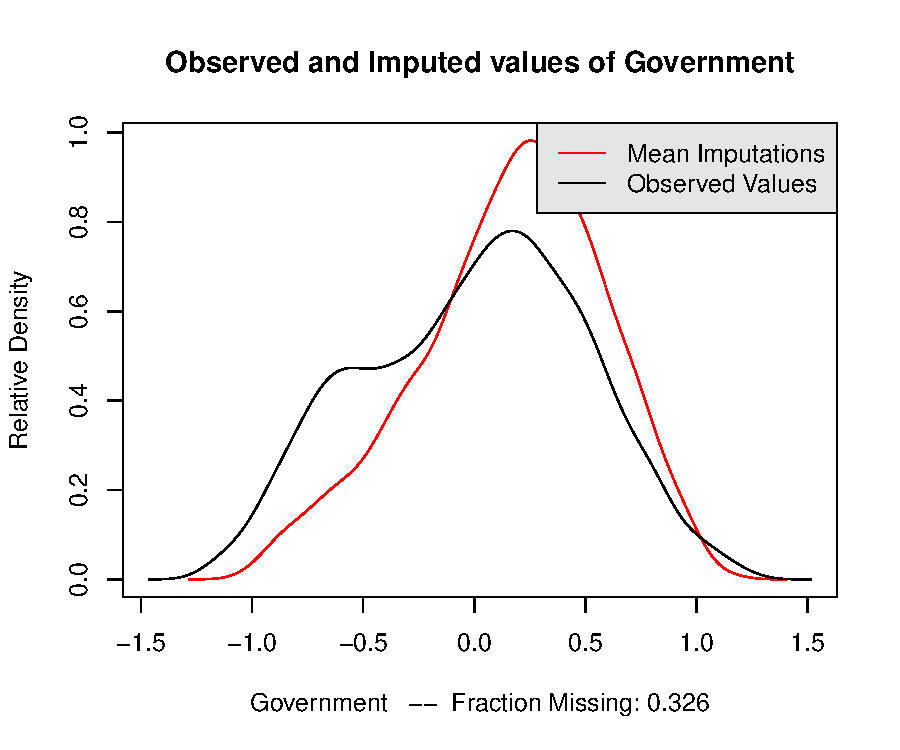
\includegraphics{figures/missing3-1.pdf}
\caption{Distributions before and after multiple imputation}
\end{figure}

\clearpage

\begin{figure}[htbp]
\centering
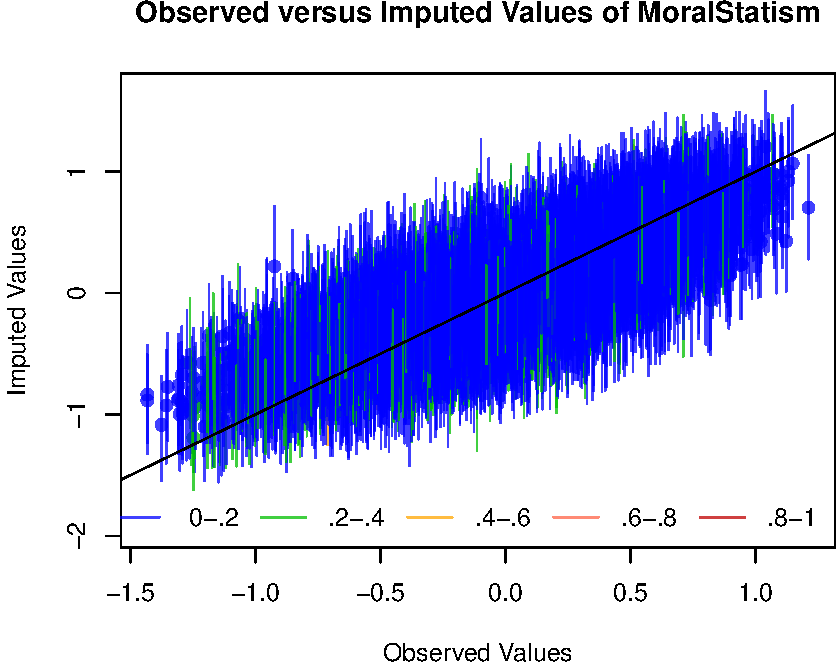
\includegraphics{figures/missing4-1.pdf}
\caption{Diagnostic Plot for Overimputation (1)}
\end{figure}

\begin{figure}[htbp]
\centering
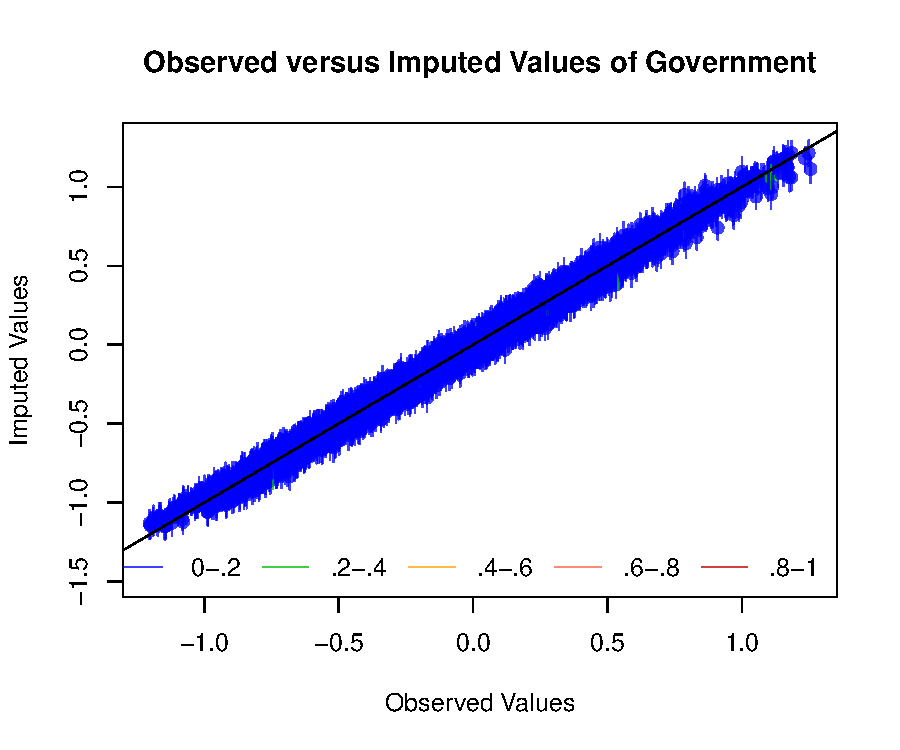
\includegraphics{figures/missing5-1.pdf}
\caption{Diagnostic Plot for Overimputation (2)}
\end{figure}

\clearpage

\begin{figure}[htbp]
\centering
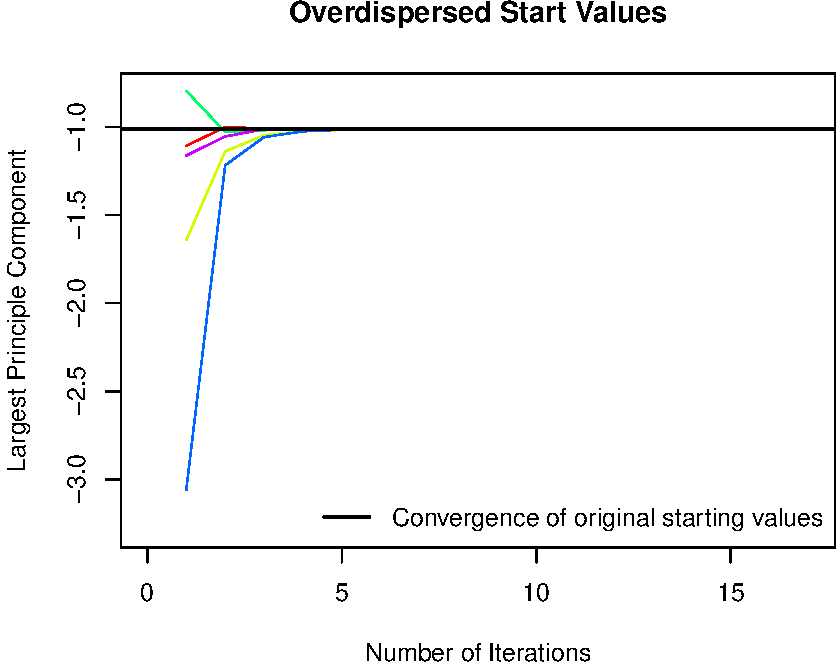
\includegraphics{figures/missing6-1.pdf}
\caption{Diagnostic Plot for Dispersion}
\end{figure}

\end{document}